\chapter{Diseño}
%\label{chapter:title}
% En caso de haber encontrado varias soluciones al problema o necesidad detectados, enumerarlas
% (Si fuera necesario realizar pruebas incluirlas como tarea en la planificación del proyecto)
\section{Gestión de alternativas}
Para solventar las necesidades de la empresa es necesario disponer de diversos servicios. Estos servicios pueden mantenerse dentro de la red local o en servidores externos bajo el mantenimiento del departamento de sistemas. Otra opción es delegar esta administración a una empresa externa bajo el modelo \textit{SaaS}\footnote{Software como Servicio. Es un modelo de negocio en el que el producto software se mantiene en la compañía que lo distribuye y mantiene y se paga por acceder mediante un cliente.}. A continuación realizaremos una lista con las posibles soluciones a rasgos generales.
\begin{itemize}
\item \textbf{Servicios autohospedados en local:} Esta solución implica la compra de un servidor físico, de torre o \textit{rackeable}, e instalarlo dentro de la red corporativa. A nivel económico, esta alternativa conlleva un gasto inicial mayor, pero luego el gasto al mes es mínimo. Al disponer de acceso físico al servidor, también es menos costoso ampliar sus capacidades.
\item \textbf{Servicios autohospedados en un VPS\footnote{Servidor Privado Virtual. Son equipos virtualizados por máquina de alto rendimiento en un CPD. Comparte recursos con los VPS de otros clientes, pero se mantiene aislado de estos.}:} El mantenimiento de los servicios seguiría estando bajo la responsabilidad de la empresa con la única diferencia de que no se tendrá acceso al servidor. Su gasto inicial es mucho menor, pero requiere de pagos mensuales para el mantenimiento.
\item \textbf{Alquiler de servicios:} No se tiene acceso al servidor, solo a los servicios que se contratan. Son bastante más baratos, pero el control es mínimo.
\end{itemize}
\subsection{Comparación de alternativas}
Como hemos dicho en la sección anterior, las opciones autohospedadas en local son las alternativas más económicas a largo plazo, pero constan de dos grandes inconvenientes:
\begin{itemize}
    \item Requieren de un mantenimiento constante. Actualizaciones y parches de seguridad en cuanto a software y supervisión de fallos y mantener la alta disponibilidad del hardware. Esto supone un gasto importante de recursos económicos y humanos a tener en cuenta.
    \item Si los datos que se manejan son esenciales o sensibles, es extremadamente peligroso mantenerlos únicamente en el servidor local. Hará falta crear una política de copias de seguridad y volcado de la información en un CPD separado por varios kilómetros. También debe tenerse en cuenta el acceso físico.
\end{itemize}

Los servicios autohospedados en un VPS son alternativas, simples y seguras. Evitas gastar recursos en la seguridad física y el volcado de datos en una réplica mientras mantienes la privacidad de tus datos y evitas restricciones y controles por parte de los proveedores de SaaS. La gran cantidad de proveedores de VPS se traduce en una mayor competitividad en los precios.

Por otro lado, el alquiler de servicios es una gran limitación al depender de productos y actualizaciones de terceros, pero reduce a casi cero el mantenimiento de la plataforma y los servidores. Los SaaS pueden dejar de ofrecer servicios o sufrir filtraciones sin que nosotros, como empresa, podamos hacer mucho; hay que vigilar el grado de dependencia de los SaaS, especialmente los privativos.

\begin{center}
\noindent\rule{5cm}{0.5pt}
\end{center}

Por último, para el acceso a la red corporativa desde cualquier dispositivo empresarial se usará una conexión VPN. Actualmente, existen dos servicios predominantes a la hora de crear una VPN.
\begin{itemize}
    \item \textbf{OpenVPN:} Creado en el 2002, es un servicio con gran recorrido, estable, configurable y bien documentado.
    \item \textbf{WireGuard:} Soportado de forma nativa por el kernel Linux, lleva desde 2018 en desarrollo y su primera versión estable salió en 2021. Tiene una seguridad criptográfica mayor que OpenVPN, es más rápido y gasta menos recursos.\cite{lipp2019mechanised}
\end{itemize}

\subsection{Selección de alternativa y justificación}
Como respuesta corta, ninguna de las soluciones propuestas es la solución preferida. La mejor opción es una combinación de dos alternativas. La gestión de los servidores de correo electrónicos y los DNS suelen ser los más problemáticos, críticos, y requieren de más recursos para su correcto funcionamiento. Por ello, se ha decidido que estos servicios se contratarán a una empresa externa junto con la gestión del almacenamiento en la nube.

Con estos nuevos requisitos, la lista de proveedores que pueden ofrecer soluciones altamente fiables se reducen drásticamente, siendo Google y Microsoft, con sus respectivas suites Workspace y Office 365, las opciones más acordes. Al tener una mejor gestión de API e integración con equipos Linux, se decide por la suite de Google.

Aunque WireGuard es una alternativa más segura y rápida, necesitaremos una opción robusta y configurable para la conexión con los equipos de los empleados a los servidores. Por ese motivo, seleccionaremos OpenVPN.

\section{Definición del proyecto}
\subsection{VPN}
% Como el proyecto va a solucionar o mejorar el problema o necesidades detectadas.
Para esta planificación vamos a crear una red VPN, usando un servidor en la nube, donde se llevará un control de todos los equipos de la empresa. Se crearán distintas subredes según el departamento desde donde se administrarán los permisos de acceso. Además, para evitar el filtrado de información, los equipos de los responsables de departamento contarán con un \textit{kill switch}, una política dentro de su cliente VPN para denegar toda conexión si no se está conectado a la VPN. Los clientes se autenticarán usando certificados y contraseña. Se usará un script llamado PiVPN (\underline{https://github.com/pivpn/pivpn}), que facilita la gestión de certificados, mantiene un inventario de direcciones IP estáticas asignadas y automatiza la creación de clientes y el revocado de certificados.
% Son los resultados deseados después de implementar el proyecto. Normalmente se definirá un objetivo principal y algunos objetivos secundarios.
\begin{figure}[H]
  \centering
  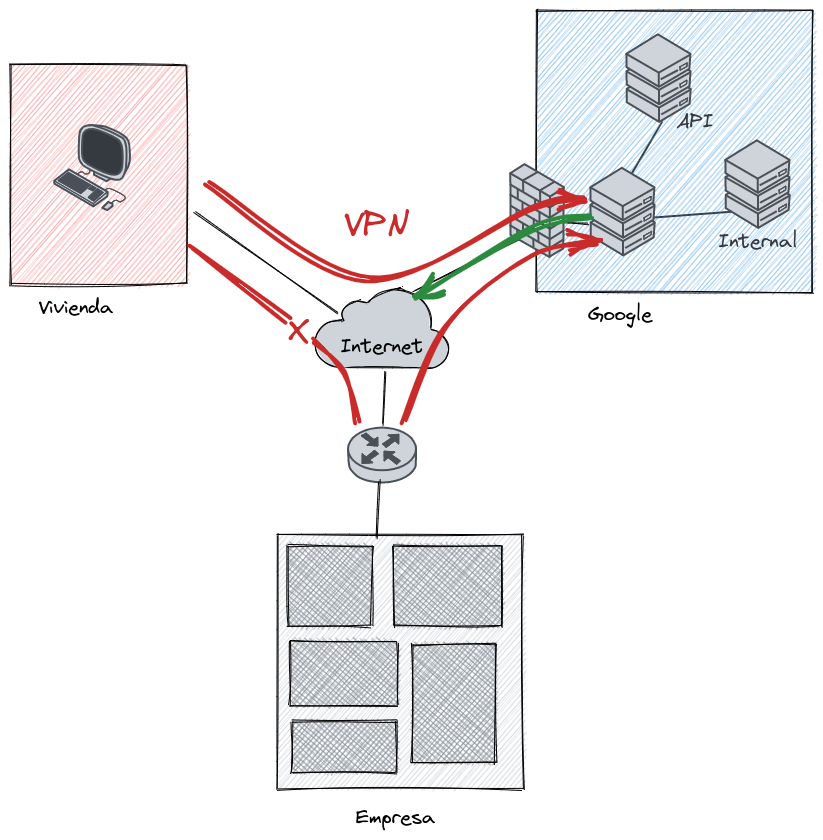
\includegraphics[width=0.5\textwidth]{figura1.png}
  \caption{Estructura VPN básica}
  \label{fig:VPNbasico}
\end{figure}

Como se puede ver en el diagrama \ref{fig:VPNbasico}, la creación de un servicio VPN nos permitirá denegar todo el acceso de equipos no identificados, los equipos clientes no podrán comunicarse entre ellos y se podrá acceder con seguridad a los recursos de la empresa desde cualquier lugar. La red VPN será global, y los distintos departamentos se organizarán por subredes, desde las que se gestionarán los permisos de acceso a los servidores. El acceso a Internet se hará a través de la VPN, esto enmascarará datos de la empresa como su ubicación física.

\subsection{Dominio y subdominios}
Por medidas de seguridad, el dominio se encontrará bajo un firewall de Cloudflare\footnote{Empresa orientada a la mitigación de ataques DDoS y enmascaramiento de los registros DNS de sus clientes bajo proxies.}. Para este proyecto usaremos el servicio gratuito, más que suficiente. Usaremos una de las tecnologías características de este servicio, el túnel. Se crea una conexión directa entre nuestros servidores y los de Cloudflare sin necesidad de abrir puertos y realizar redirecciones. En los registros DNS aparecen las IP de Cloudflare, y estos son los encargados de redirigir el tráfico indicándole la IP y el puerto que deseamos, igual que con un proxy inverso\cite{CloudflareTunnel}.

\subsubsection{Estructura}
En total, dispondremos de un solo dominio, el que ya hemos comentado, y algunos subdominios:
\begin{itemize}
    \item \textbf{[REDACTADO].es}: Dominio principal, contiene la página web de la empresa, no incumbe en este proyecto.
    \item \textbf{api.[REDACTADO].es}: Subdominio público, pone en contacto a los desarrolladores externos con el acceso público de uno de los servidores.
    \item \textbf{internal.[REDACTADO].es}: Subdominio privado, hospeda el portal del empleado, documentación interna, etcétera. Solo será accesible desde la VPN.
\end{itemize}
\subsection{Redes y control de acceso}
Al existir la posibilidad de cambiar de puesto constantemente, la posibilidad de gestionar los accesos a través de la red interna queda descartada. En su lugar, se hará a través de la VPN, lo que obligará a los usuarios a mantenerse conectados para poder trabajar. Cada departamento se separará por subredes:
\begin{table}[h!]
\centering
\begin{tabular}{|c|c|c|}
\hline
Equipo         & Red         & Acceso      \\ \hline
Servidores     & 10.218.0.0/24       & Nada        \\ \hline
Sistemas     & 10.218.1.0/24       & Todo        \\ \hline
Backend      & 10.218.2.0/24        & API e Interno       \\ \hline
Frontend       & 10.218.3.0/24       & Principal e Interno        \\ \hline
UI/UX         & 10.218.4.0/24          & Principal e Interno        \\ \hline
Diseño gráfico       & 10.218.5.0/24 & Interno        \\ \hline
Contabilidad & 10.218.6.0/24   & Interno        \\ \hline
Ventas   & 10.218.7.0/24         & Interno        \\ \hline
Gerente      & 10.218.8.0/24        & Todo        \\ \hline
\end{tabular}
\label{tab:tabla_personal}
\end{table}
\subsection{Google}
Dentro del ecosistema de Google tendremos tres servidores: Principal, API e Interno. El acceso estará restringido por red y requerirá autentificación del usuario. Un firewall de Google será el encargado de la comunicación entre el exterior y los servidores.
% Resumen de las tareas necesarias para llevar a cabo el proyecto (p. ej. podrían ser: diseño, planificación y desarrollo) que luego se detallan y temporalizan en el apartado 3.3